\section{System Design}\label{c:sdd}

\subsection{Architecture}

The system is layered so the compiler core has no knowledge of the web application around
it. \texttt{core/} depends on nothing but the standard library and pydantic and can be
exercised from the command line; the API is a thin translation between HTTP and core
calls; the database stores corpus records only.

\diagram{architecture.png}{0.78}{System architecture. The compiler core is independent of
the service and interface layers surrounding it.}

\begin{keypoint}[Derived analysis is never stored]
The database holds statements, not results. Every analysis is recomputed on request from
the current grammar and lexicon, so a specification change can never leave stale verdicts
behind --- which, in a document generated from live data, is the difference between a
correct report and a quietly wrong one (\req{NFR-2}, \req{NFR-8}).
\end{keypoint}

\subsection{Module decomposition}

\begin{center}
\scriptsize
\begin{tabular}{@{}l l p{5.0cm} l@{}}
\toprule
\textbf{Layer} & \textbf{Module} & \textbf{Responsibility} & \textbf{Satisfies} \\
\midrule
\multirow{9}{*}{\rotatebox{90}{\textbf{Compiler core}}}
 & \texttt{core/text.py}     & Scanning, canonicalisation, accent folding   & \req{FR-9}, \req{FR-15} \\
 & \texttt{core/lexer.py}    & Tokenisation, lexicon resolution             & \req{FR-11}--\req{FR-14}, \req{FR-16} \\
 & \texttt{core/lexicon.py}  & Entry storage, lookup indices, homographs    & \req{FR-12}, \req{FR-15} \\
 & \texttt{core/grammar.py}  & Grammar model, transformations, ledger       & \req{FR-18}--\req{FR-21} \\
 & \texttt{core/ll1.py}      & FIRST/FOLLOW, table construction             & \req{FR-22}, \req{FR-23} \\
 & \texttt{core/parser.py}   & Predictive parser                            & \req{FR-24}--\req{FR-26} \\
 & \texttt{core/suggest.py}  & Deterministic repair suggestions             & \req{FR-27} \\
 & \texttt{core/analysis.py} & Snapshots, frequencies, topic matching       & \req{FR-17}, \req{FR-32} \\
 & \texttt{core/corpus.py}   & Validation, revisions, provenance            & \req{FR-1}--\req{FR-7} \\
\midrule
\multirow{2}{*}{\rotatebox{90}{\textbf{Svc}}}
 & \texttt{api/main.py}      & Application factory, middleware              & \req{NFR-5} \\
 & \texttt{api/routes/}      & analysis, auth, corpus, export, grammar, statistics & \req{FR-8}, \req{FR-28}--\req{FR-31} \\
\midrule
\multirow{2}{*}{\rotatebox{90}{\textbf{UI}}}
 & \texttt{cli.py}           & Offline analysis, seeding, provisioning      & \req{FR-24} \\
 & React front end           & Analyser, grammar explorer, corpus manager   & \req{FR-28}--\req{FR-32} \\
\bottomrule
\end{tabular}
\end{center}

\subsection{Processing pipeline and domain model}

Each stage is a pure function over immutable data: \texttt{scan} $\rightarrow$
\texttt{lex} $\rightarrow$ \texttt{prepare} $\rightarrow$ \texttt{parse} $\rightarrow$
\texttt{analyse}. No stage mutates its input, so a snapshot is exactly reproducible from
the statement text plus the grammar and lexicon versions stamped into it (\req{NFR-1}).

\begin{figure}[htbp]
  \centering
  \begin{minipage}[c]{0.49\linewidth}
    \centering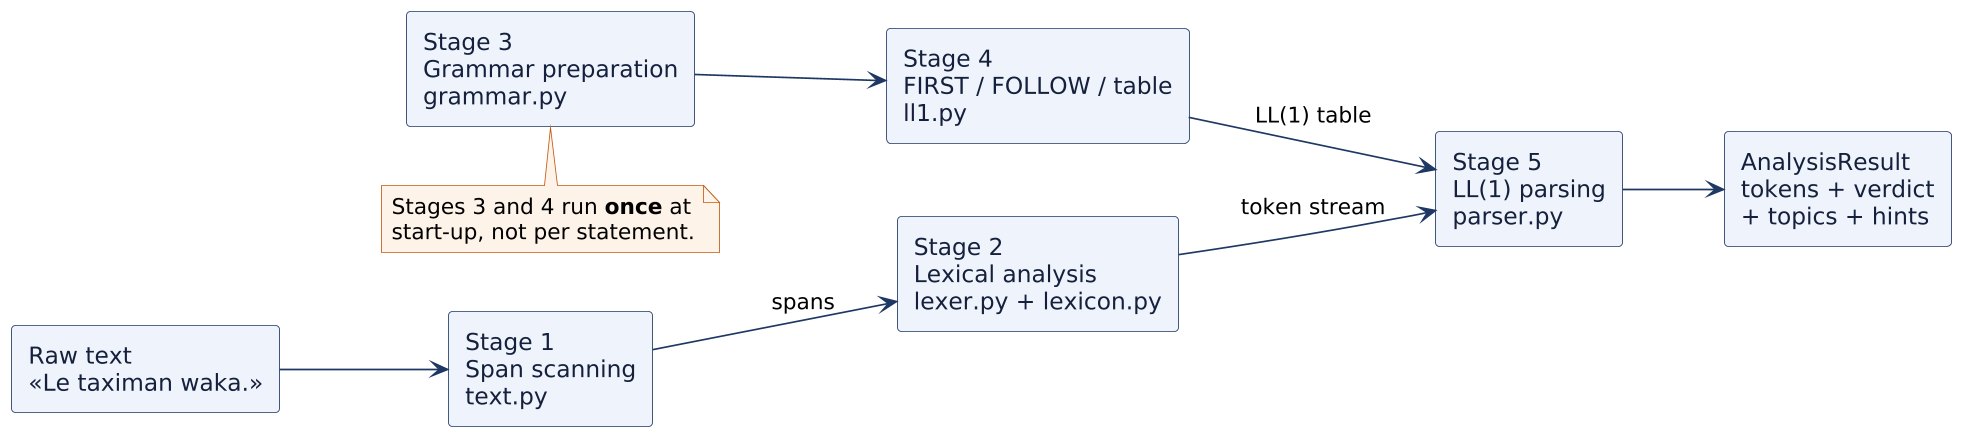
\includegraphics[width=\linewidth]{figures/pipeline.png}
  \end{minipage}\hfill
  \begin{minipage}[c]{0.46\linewidth}
    \centering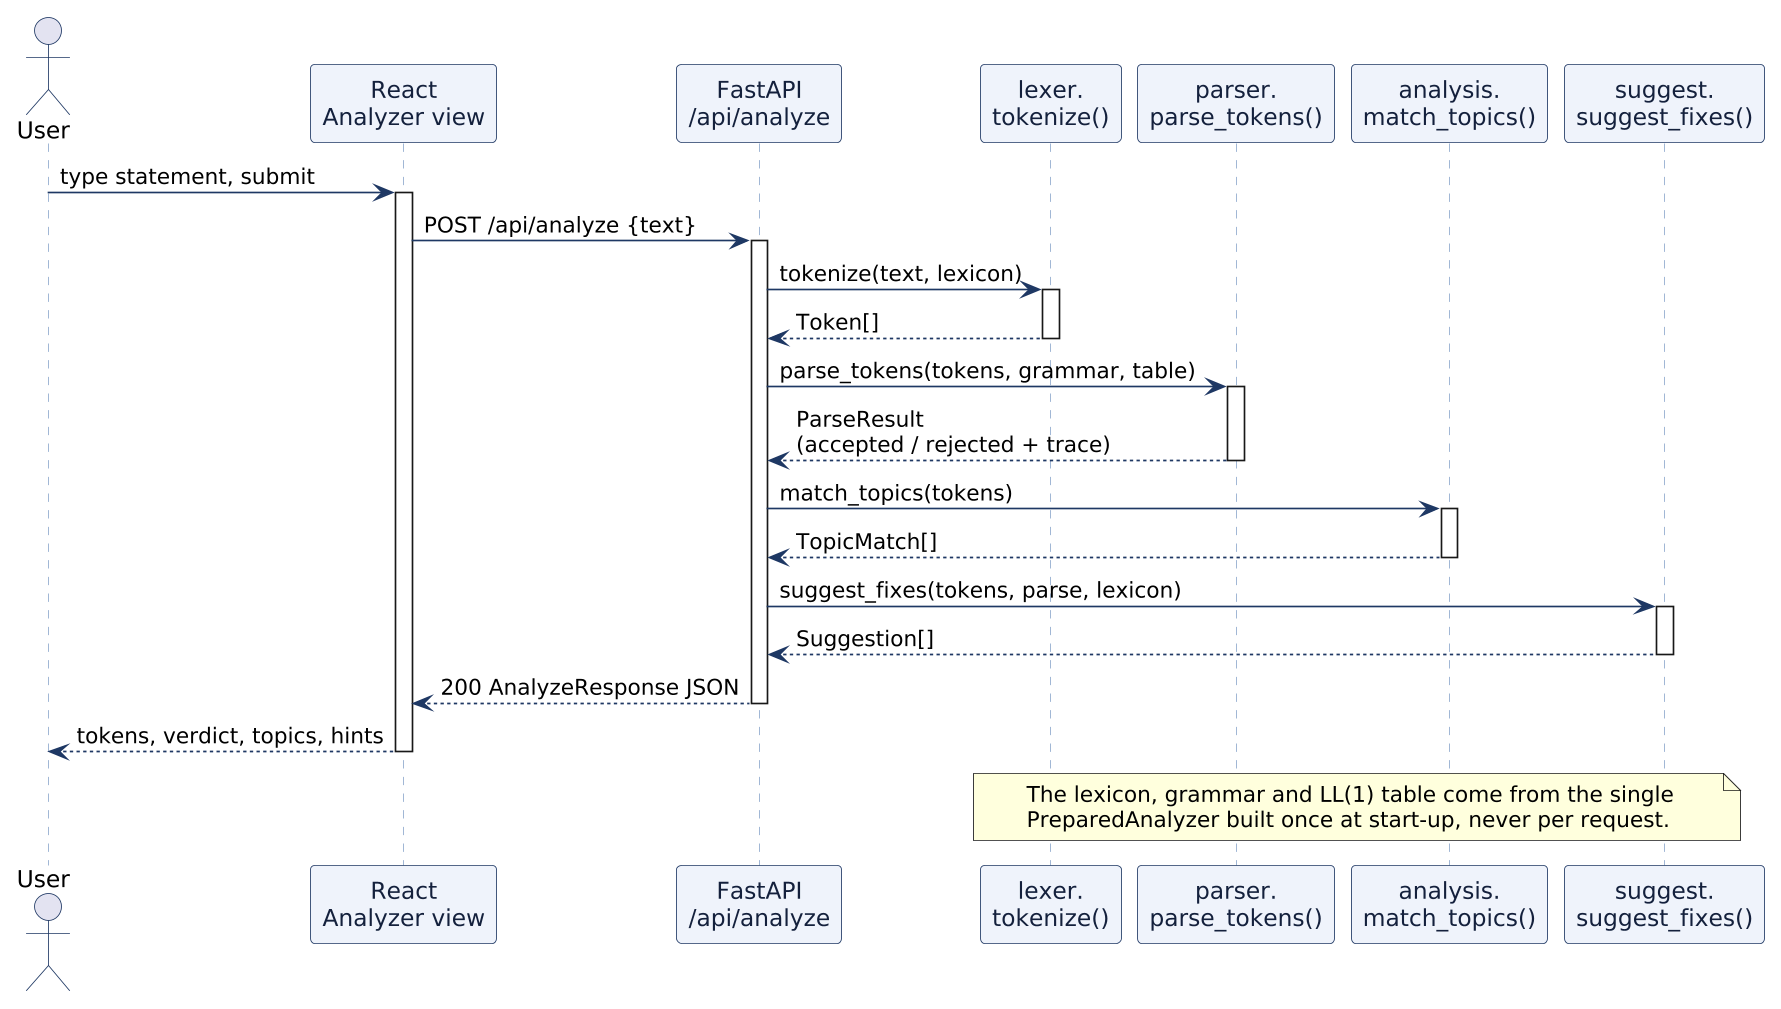
\includegraphics[width=\linewidth]{figures/sequence-analyze.png}
  \end{minipage}
  \caption{Left: the five-stage analysis pipeline. Right: an analyse request travelling
  from the browser through the API to the parser and back.}
  \label{fig:pipeline-sequence}
\end{figure}

All domain types are frozen pydantic models that refuse unknown fields (\req{NFR-4}). A
mistyped field name therefore raises at construction time rather than silently producing
a snapshot with a missing attribute --- in a data-analysis pipeline, the difference between
a crash and a wrong number in this report.

\subsection{Data design}

\begin{center}
\scriptsize
\begin{tabular}{@{}l p{9.9cm}@{}}
\toprule
\textbf{Table} & \textbf{Purpose and key columns} \\
\midrule
\texttt{users}                & Collector accounts; Argon2 password hashes. \\
\texttt{auth\_sessions}       & Server-side sessions with CSRF tokens and expiry. \\
\texttt{statement\_records}   & Statement identity; pointer to the currently published revision. \\
\texttt{statement\_revisions} & Append-only revisions: raw text, source kind, attestation flag, collector, topics, timestamp. \\
\texttt{analysis\_snapshots}  & Optional persisted results, pinned to one exact revision and specification hash. \\
\bottomrule
\end{tabular}
\end{center}

Separating \emph{identity} from \emph{revision} is what makes \req{FR-6} enforceable: a
record's history is a list of immutable rows, and publication is a pointer into that list
rather than a mutable flag on the statement itself. Lexicon, grammar and corpus are
versioned JSON specifications bundled inside the installed package, so the deployed
service and the local test suite load byte-identical data.

\subsection{Security and deployment}

Authentication uses Argon2 hashing with opaque server-side session tokens. Session
cookies are \texttt{HttpOnly}, \texttt{Secure} in production and \texttt{SameSite=Lax}; a
double-submit CSRF token is required on every state-changing request, and requests that
predate a session must pass a same-origin check. The container runs as a non-root,
non-login user with only the data volume writable, and its port binds to loopback behind
an Nginx reverse proxy that terminates TLS and serves the built single-page application.
The browser therefore sees one origin, so cookies work without relaxing \texttt{SameSite}.

\subsection{Key design decisions}

\begin{center}
\scriptsize
\begin{tabular}{@{}p{3.3cm} p{3.9cm} p{4.9cm}@{}}
\toprule
\textbf{Decision} & \textbf{Alternative rejected} & \textbf{Rationale} \\
\midrule
Hand-written lexer and parser & \texttt{lex}/\texttt{yacc} or a generator &
  The transformations are the assessed work; generating them hides the reasoning. \\
Author the grammar left-recursively & Write it pre-factored &
  Pre-factoring by hand produces an empty ledger and loses the evidence for \req{FR-21}. \\
Donor language per \emph{token} & Per statement &
  Speakers switch mid-clause, so no span of text holds a single language. \\
Folding as a fallback tier & Fold everything by default &
  Folding collapses four attested homograph pairs differing only by a diacritic. \\
Recompute analysis on request & Cache derived results &
  A specification change can never leave a stale verdict published. \\
\bottomrule
\end{tabular}
\end{center}
